\documentclass[11pt]{article}
\usepackage[utf8]{vietnam}
\usepackage{hyperref}
\usepackage{makecell}
\usepackage{blindtext}
\usepackage{xcolor}
\usepackage{enumitem}
\usepackage{listings}
\hypersetup{
    colorlinks=true, 
    linkcolor=blue,
    filecolor=magenta,      
    urlcolor=red,
    pdftitle={Overleaf Example},
    pdfpagemode=FullScreen,
    }
\usepackage{amsmath,amssymb,amsfonts}
\usepackage{graphicx}

\setlength{\topmargin}{-.5in} \setlength{\textheight}{9.25in}
\setlength{\oddsidemargin}{0in} \setlength{\textwidth}{6.8in}

%%%%%%%%%%%%%%%%%%%%%%%%%%%%%%%%%%%%%%%%%%
% \usepackage{pythonhighlight}
%%%%%%%%%%%%%%%%%%%%%%%%%%%
\newcounter{mycounter} % create a new counter, called 'mycounter'
% default def'n of '\themycounter' is '\arabic{mycounter}'
%% command to increment 'mycounter' by 1 and to display its value:
\newcommand\showmycounter{\stepcounter{mycounter}\themycounter}
\usepackage{lipsum}
\newcommand\showlips{\stepcounter{mycounter}\lipsum[\value{mycounter}]}
%%%%%%%%%%%%%%%%%%%%%%%%%%%%%%%%%%%%%%
\usepackage{framed}
\usepackage{hyperref}
\usepackage{fancyhdr}

%%%%%%%%%%%%%%%%%%%%%%%%%%%%%%%%%%%%%%%%%%%%%%%%%%%%%%%%%%%%%
\usepackage{listings}
\usepackage{xcolor}

\definecolor{codegreen}{rgb}{0,0.6,0}
\definecolor{codegray}{rgb}{0.5,0.5,0.5}
\definecolor{codepurple}{rgb}{0.58,0,0.82}
\definecolor{backcolour}{rgb}{0.95,0.95,0.92}

\lstdefinestyle{mystyle}{
    backgroundcolor=\color{backcolour},   
    commentstyle=\color{codegreen},
    keywordstyle=\color{magenta},
    numberstyle=\tiny\color{codegray},
    stringstyle=\color{codepurple},
    basicstyle=\ttfamily\footnotesize,
    breakatwhitespace=false,         
    breaklines=true,                 
    captionpos=b,                    
    keepspaces=true,                 
    numbers=left,                    
    numbersep=5pt,                  
    showspaces=false,                
    showstringspaces=false,
    showtabs=false,                  
    tabsize=2
}

\lstset{style=mystyle}
%%%%%%%%%%%%%%%%%%%%%%%%%%%%%%%%%%%%%%%%%%%%%%%%%%%%%%%%%%%%%
\title{\LARGE AI VIET NAM – COURSE 2024}
\author{\Huge \begin{minipage}{\textwidth}\centering Hướng dẫn chia sẻ và phân quyền trong Figma \end{minipage}}
\pagestyle{fancy}
\fancyhf{}
\lhead{\bfseries AI VIETNAM}
\rhead{\bfseries  aivietnam.edu.vn}
\begin{document}
\maketitle

\textbf{Nguồn dữ liệu:} \href{https://help.figma.com/hc/en-us/sections/1500001331382-Sharing-and-permissions}{figma.com}

\section{Giới thiệu}

Trong Figma, bạn có thể chia sẻ nhiều loại khác nhau như: dự án, tệp hay một vài thành phần trong dự án.
\begin{figure}[!h]
    \centering
    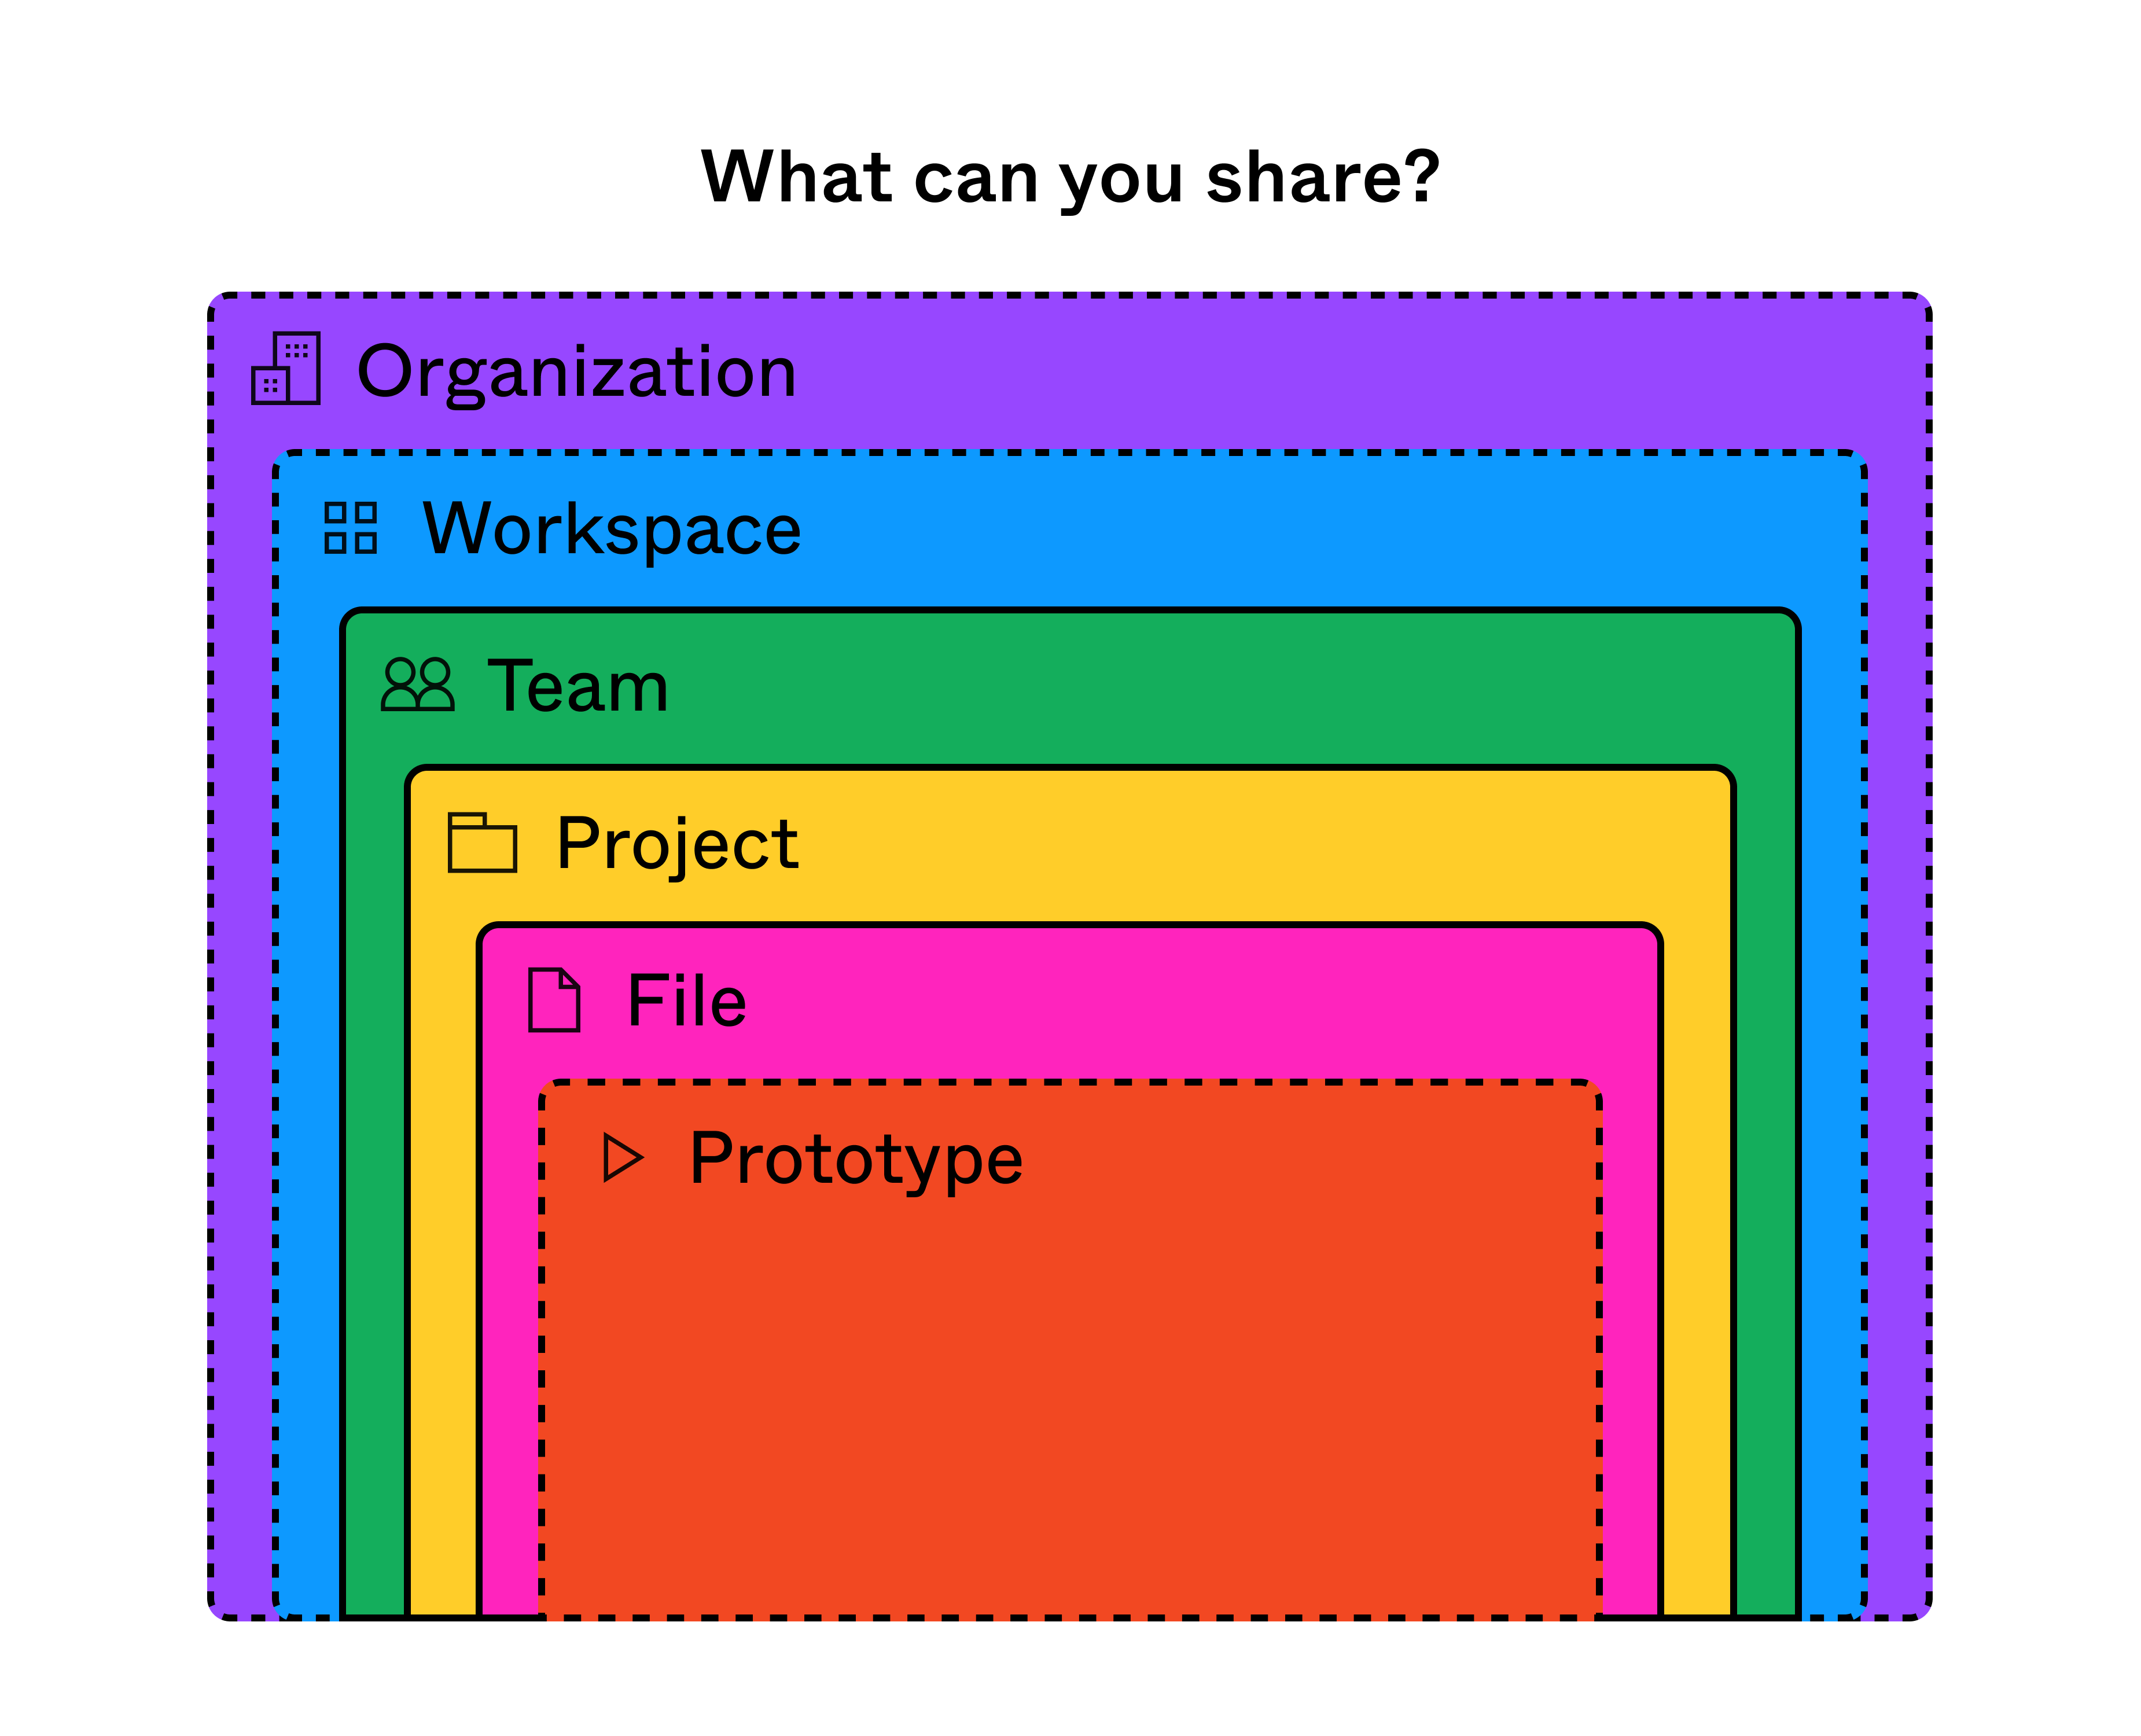
\includegraphics[width=0.8\linewidth]{imgs/share.png}
    \caption{Cơ cấu tổ chức trong Figma}
\end{figure}

Thông thường, việc cấp quyền cho ai đó quyền truy cập ở một cấp độ sẽ cho phép họ truy cập đến cấp độ thấp hơn. Chúng ta có 3 cách để chia sẻ các đối tượng:

\begin{itemize}
    \item Chia sẻ liên kết: mỗi tệp và nguyên mẫu sẽ có 1 URL duy nhất. Tiến hành sao chép
    \item Mời mọi người cộng tác thông qua tài khoản, email: nhập địa chỉ email của họ để mời họ tham gia.
    \item Nhúng tệp hoặc nguyên mẫu (prototype) ra bên ngoài Figma
\end{itemize}

\section{Chia sẻ}
Chia sẻ giúp bạn có thể quyết định được ai có thể truy cập vào tệp hay các đối tượng trong dự án của mình. Cách thực hiện:


\begin{itemize}
    \item Mở hoặc tạo mới tệp
    \item Nhấp vào "Share" trên thanh công cụ

          \begin{figure}[!h]
              \centering
              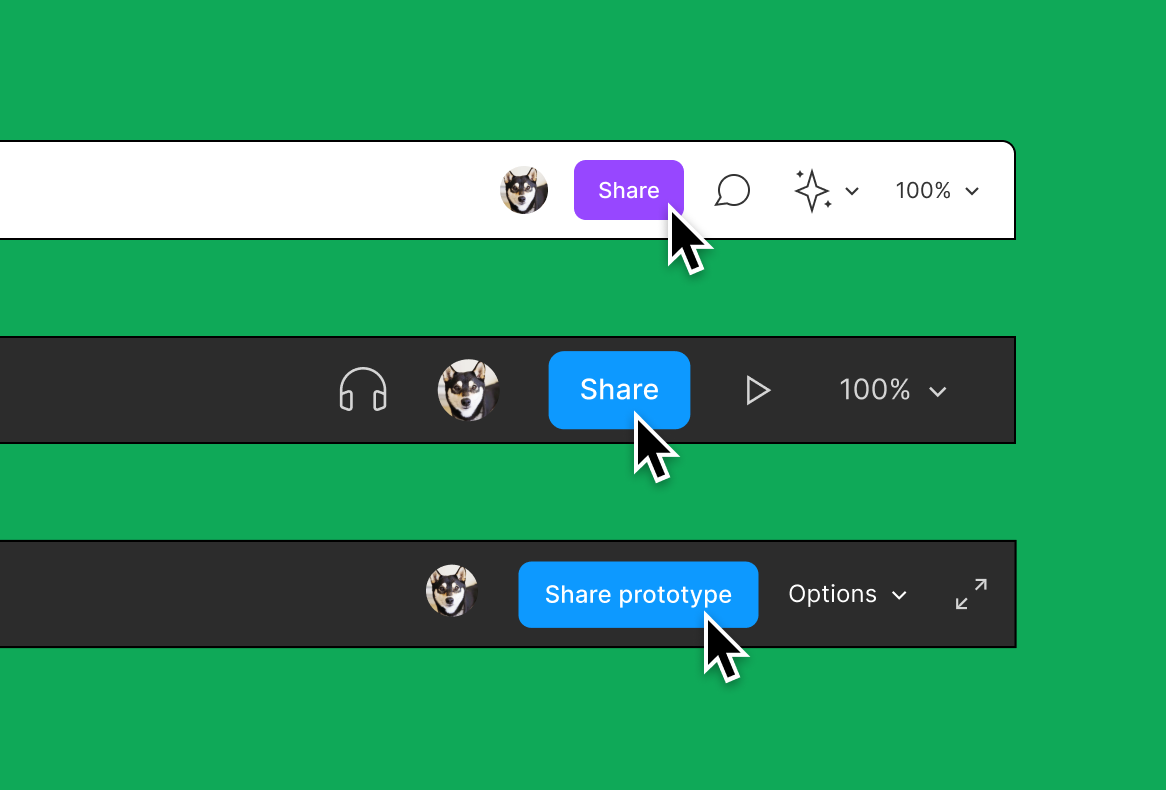
\includegraphics[width=1\linewidth]{imgs/1.png}
              \caption{Chia sẻ}
          \end{figure}

          \newpage

    \item Từ hộp thoại Chia sẻ, bạn có thể truy cập vào phần cài đặt phân quyền:

          \begin{figure}[!h]
              \centering
              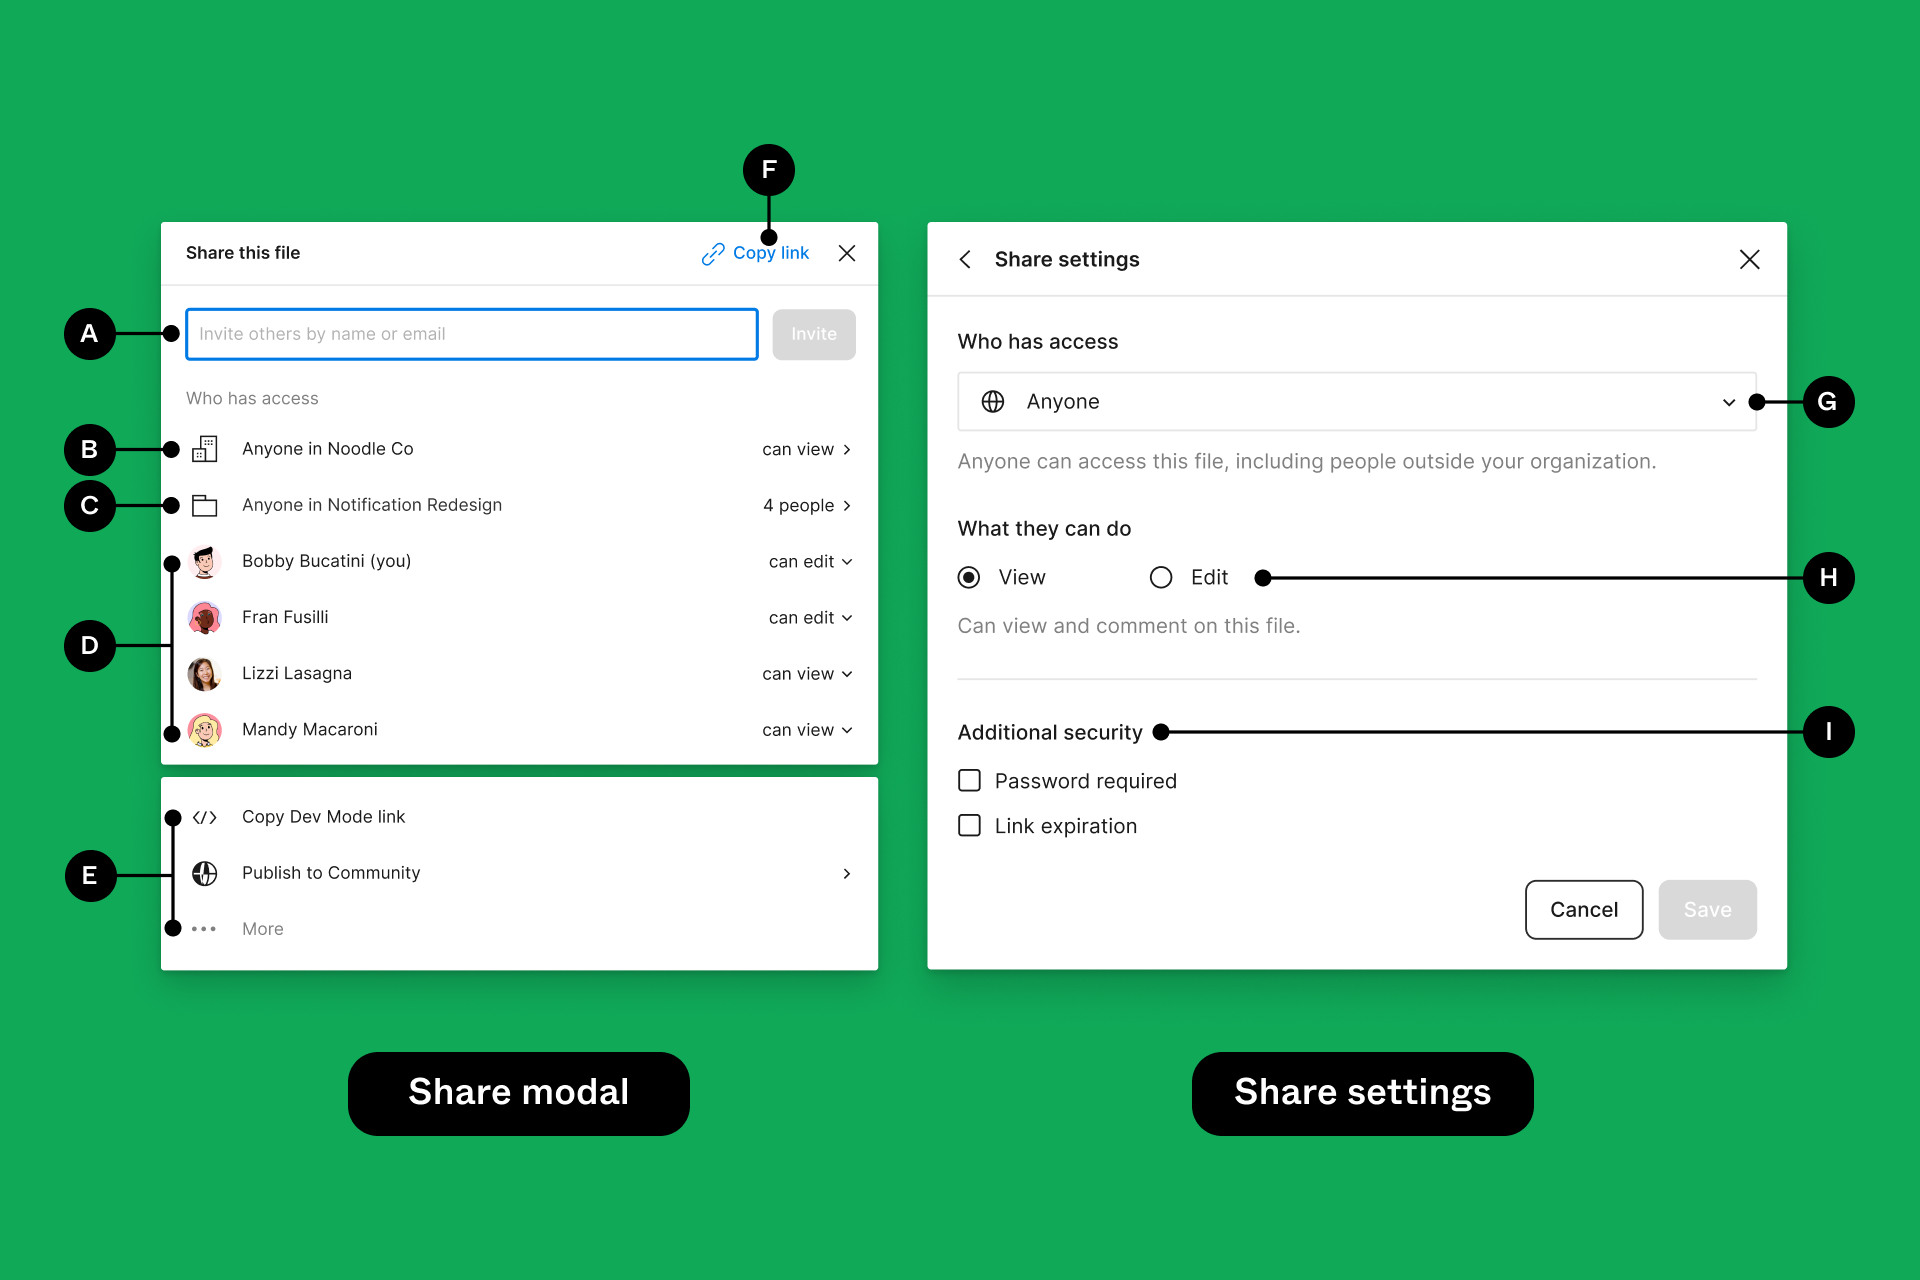
\includegraphics[width=1\linewidth]{imgs/2.png}
              \caption{Phân quyền}
          \end{figure}

          \begin{itemize}
              \item A: Nơi điền thông tin tên người dùng hoặc email của người bạn muốn mời cộng tác
              \item B: Quyền chia sẻ hiện tại của tệp. Nhấp vào để điều chỉnh quyền cụ thể của người dùng như: chỉ có quyền xem hay có thể sửa.
              \item G: Cài đặt đối tượng truy cập
              \item H: Quyền cụ thể của từng đối tượng
              \item I: Nâng cao (gói trả phí)
              \item C: Quyền của dự án
              \item D: Danh sách người dùng đang có quyền tại tệp hiện tại.
              \item E: Tuỳ chọn chia sẻ: sao chép liên kết, nhúng vào code,...
              \item F: Sao chép liên kết
          \end{itemize}


\end{itemize}
\newpage
\section{Phân quyền truy cập}

\begin{figure}[!h]
    \centering
    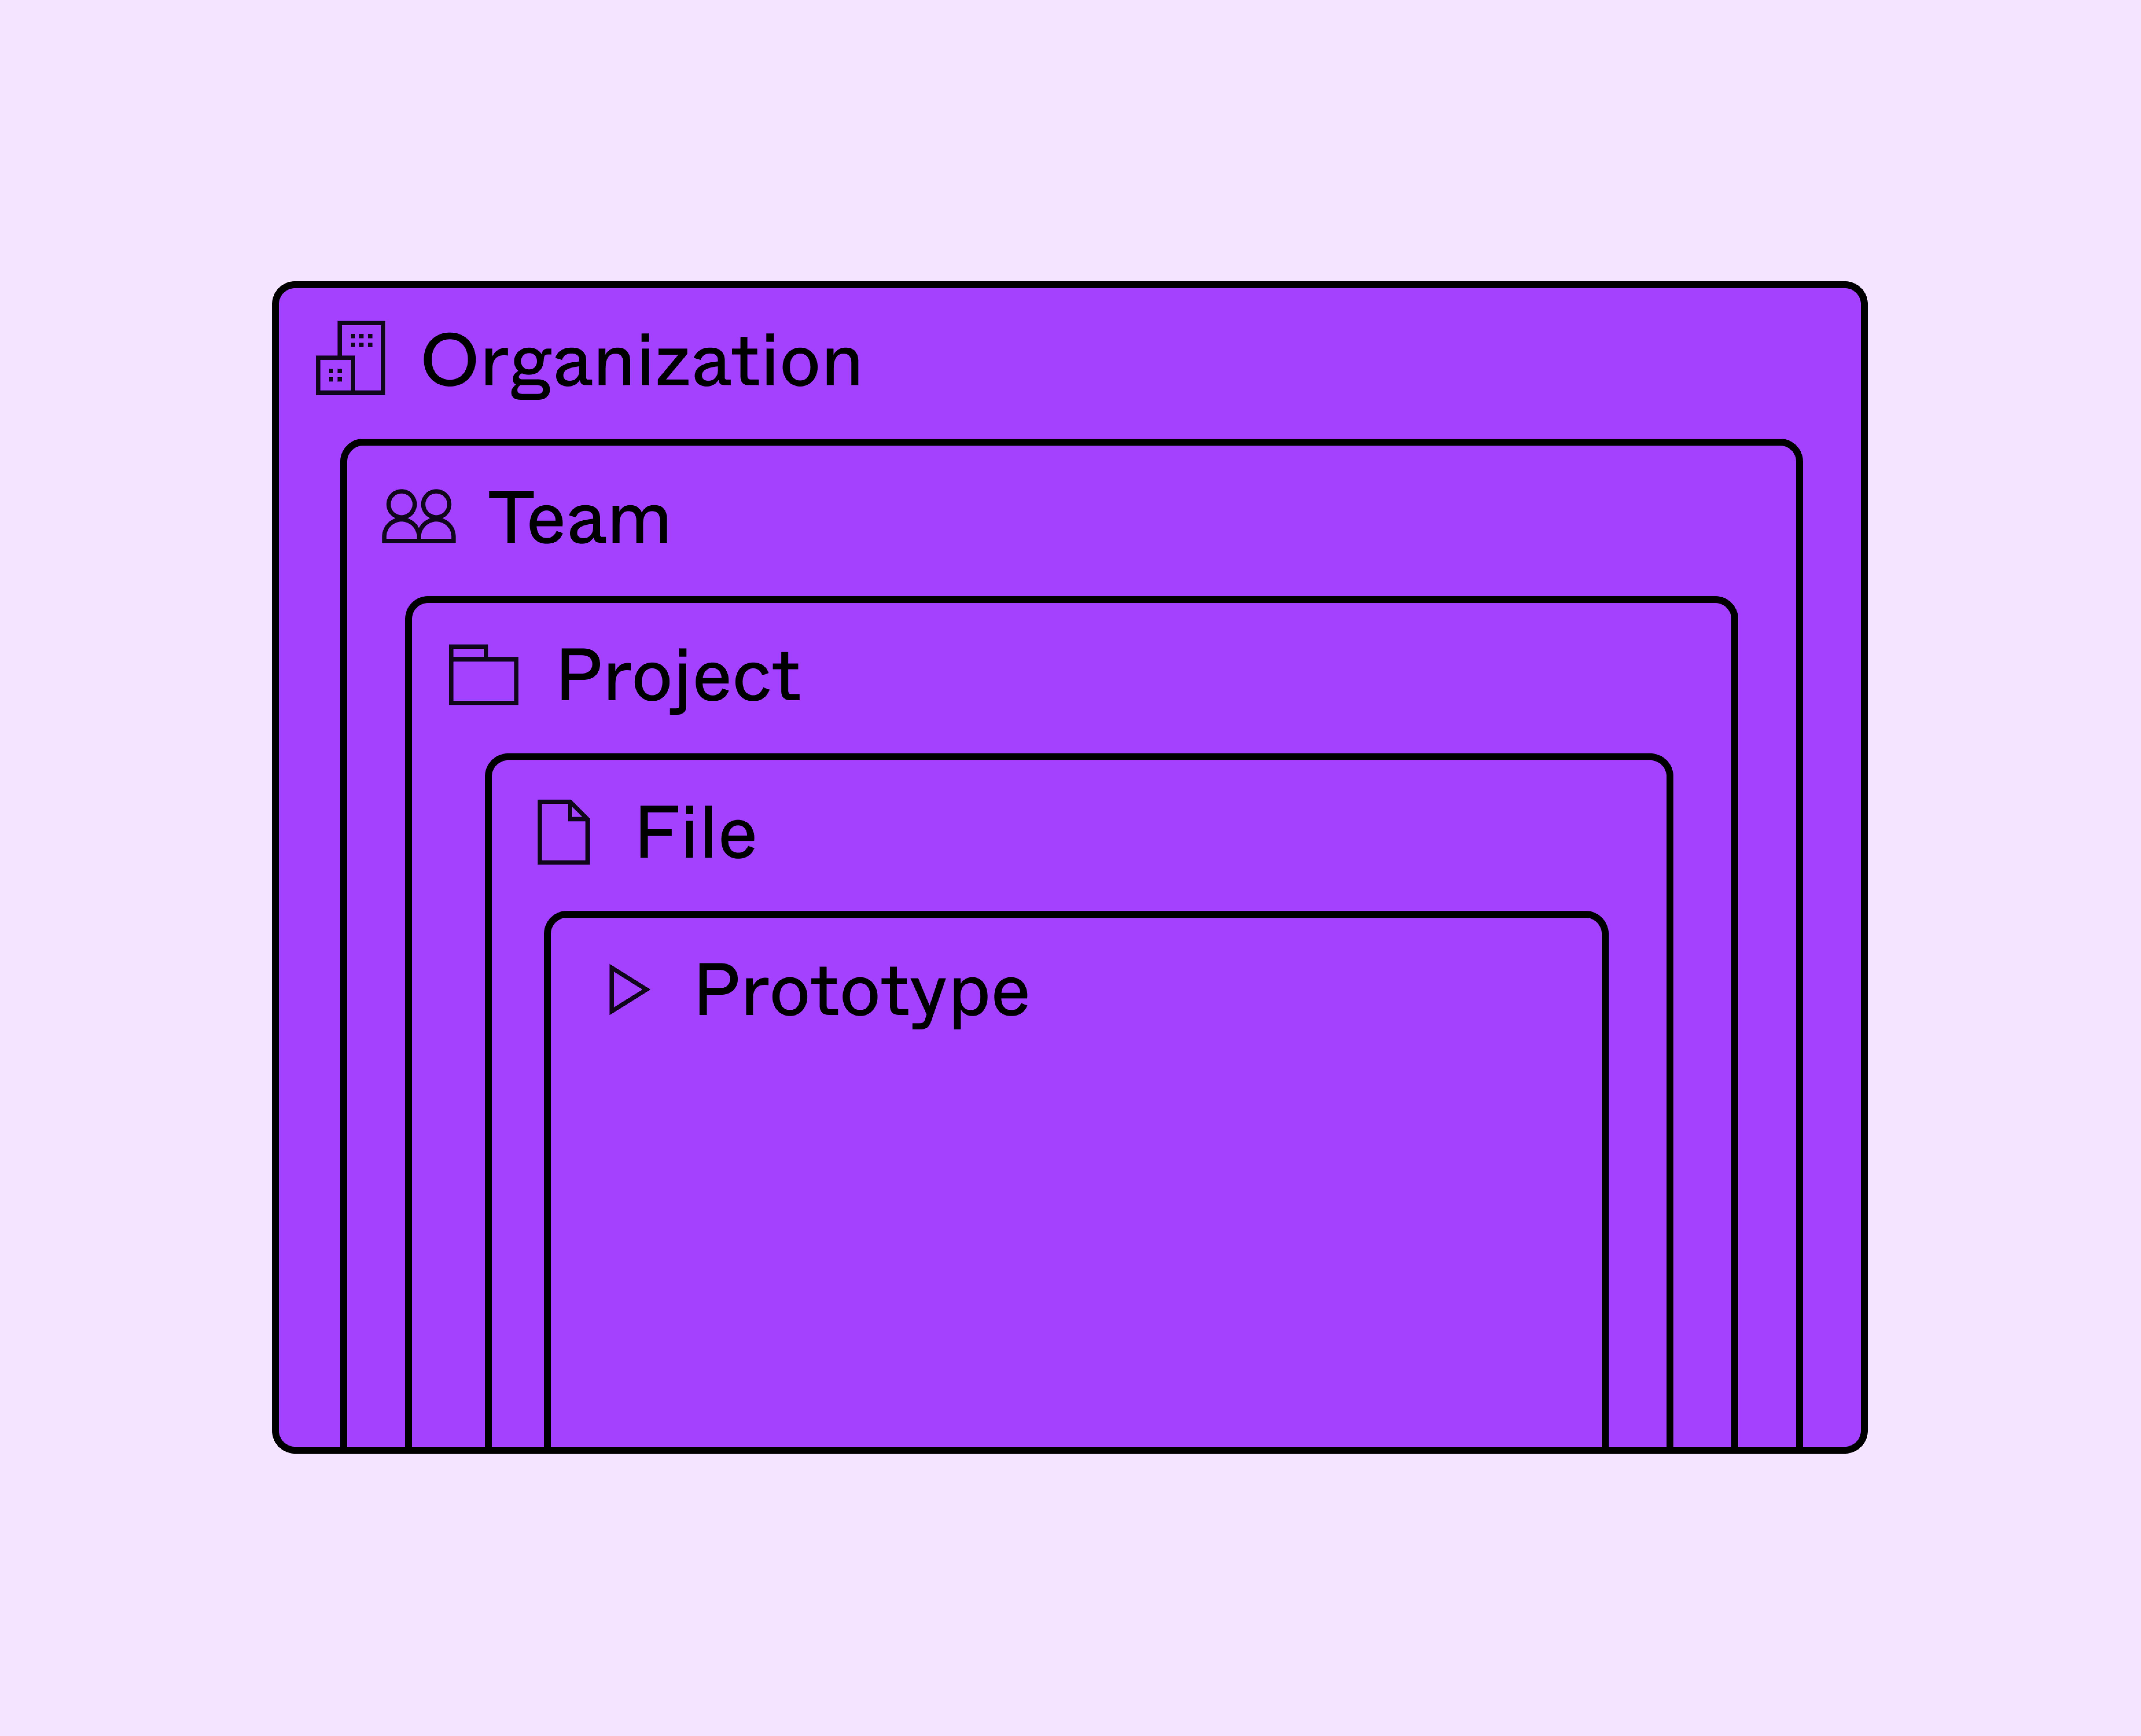
\includegraphics[width=1\linewidth]{imgs/3.png}
    \caption{Các sắp xếp tệp trong Figma}
\end{figure}

\begin{figure}[!h]
    \centering
    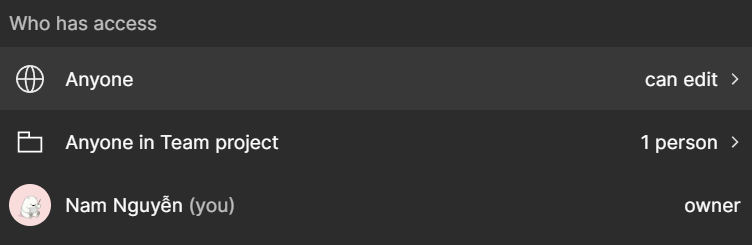
\includegraphics[width=1\linewidth]{imgs/4.png}
    \caption{Phân quyền}
\end{figure}

Theo mặc định, mỗi cấp con kế thừa từ các cấp cha của chúng. Nhưng ta có thể thay đổi trên bất kỳ cấp nào, quyền được thiết lập sẽ ghi đè lên quyền kế thừa cũ. Ta cũng có thể phân quyền cho từng người riêng biệt với những quyền khác nhau. Ta có các cấp độ truy cập như sau:

\begin{itemize}
    \item Who has access: xác định ai có quyền truy cập vào tệp
          \begin{itemize}
              \item Anyone: bất kỳ ai đều có quyền truy cập
              \item Organization name]: bất kỳ ai trong tổ chức đều có quyền truy cập.
              \item Only invited people: chỉ những người được mời trực tiếp mới có quyền truy cập.
          \end{itemize}

    \item Permission
          \begin{itemize}
              \item Can edit: cho phép người dùng chỉnh sửa tệp.
              \item Can view: người dùng chỉ có quyền xem, không được chỉnh sửa.
          \end{itemize}
\end{itemize}


\section{Kết luận}
% \item
%       \textbf{Kết luận}
Figma là một công cụ mạnh mẽ cho thiết kế giao diện người dùng và cộng tác trực tuyến. Với các chức năng đa dạng, phím tắt hữu ích, và khả năng tích hợp plugin mạnh mẽ, Figma giúp các nhà thiết kế tạo ra những sản phẩm chất lượng cao và tối ưu hóa quy trình làm việc. Hy vọng rằng tài liệu hướng dẫn này sẽ giúp ta nắm bắt và sử dụng Figma một cách hiệu quả nhất.



% \end{enumerate}

\centering{\LARGE ---------Hết---------}


\end{document}